\textit{Dans ce problème, les figures qui sont dessinées ne sont pas représentées à l’échelle.}

\subsection*{Partie A : Installation du potager}

Une enseignante a le projet d’installer un potager rectangulaire $ADEF$ sur une parcelle de
forme triangulaire $ABC$ dans l’enceinte de l’école.

Les points $A$, $B$, $C$, $D$, $E$ et $F$ sont tels que :
\begin{list}{$\bullet$}{}
    \item $AB = 24$ m, $AC = 10$ m et $BC = 26$ m ;
    \item $D \in [AB]$, $E \in [BC]$ et $F \in [AC]$.
\end{list}

\begin{center}
    \begin{tikzpicture}[x=1cm,y=1cm]        
        \draw (-5,-4) -- (4,-1) -- (-7,2) -- cycle;
        \draw[pattern=north east lines,pattern color=black] (-6.653,0.959) -- (-5.0915,1.4795) -- (-3.4385,-3.4795) -- (-5,-4) -- cycle;
        \draw (-5,-4)-- (4,-1);
        \draw (4,-1)-- (-7,2);
        \draw (-7,2)-- (-5,-4);
        \draw (-6.653,0.959)-- (-5.0915,1.4795);
        \draw (-5.0915,1.4795)-- (-3.4385,-3.4795);
        \begin{scriptsize}        
        \draw (-5.2,-4.2) node {$A$};        
        \draw (4.2,-1.2) node {$B$};
        \draw (-7.3,2) node {$C$};        
        \draw (-7,0.8) node {$F$};        
        \draw (-4.9,1.8) node {$E$};        
        \draw (-3.3,-3.8) node {$D$};
        \end{scriptsize}
    \end{tikzpicture} 

    \textit{La figure ci-dessus n’est pas à l’échelle.}       
\end{center}

\begin{enumerate}
    \item Montrer que le triangle $ABC$ est rectangle en $A$.
    
    Dans la suite de cette partie, on souhaite déterminer où positionner le point $D$ sur $[AB]$ pour
    que l’aire du rectangle hachuré $ADEF$ soit la plus grande possible.
    \item Dans cette partie on considère que $AD = 4,8$ m.
    \begin{enumerate}
        \item Montrer que la longueur $DE$ est égale $8$ m.
        \item En déduire l'aire du rectangle $ADEF$ en m\up{2}.
        
        On note $x$ la longueur, exprimée en mètre, du segment $[AD]$.
    \end{enumerate}
    \item 
    \begin{enumerate}
        \item Montrer que $DE = 10 -\dfrac{5}{12}x$.
        \item En déduire l'aire du rectangle $ADEF$ en fonction de $x$.
    \end{enumerate}
    \clearpage
    \item Le graphique ci-dessous représente l'aire, exprimée en mètre carré, du rectangle $ADEF$
    en fonction de la longueur $x$ en mètre.
    \begin{center}
        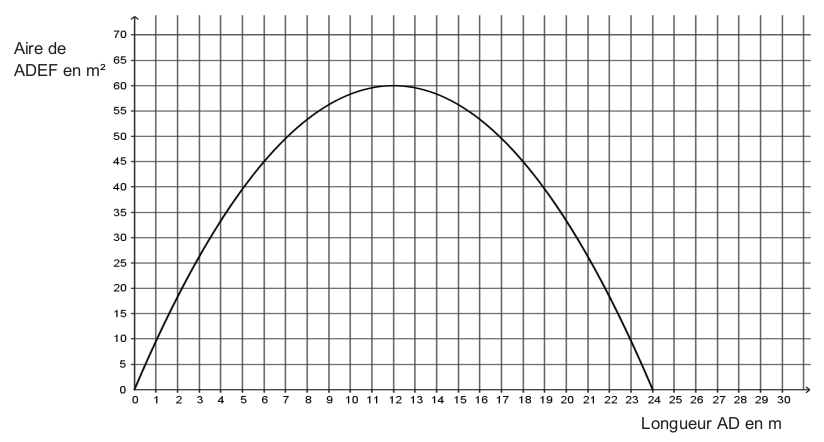
\includegraphics[width=0.95\textwidth]{./images/2022-g3-ex3-img1.png}
    \end{center}

    À l'aide du graphique, répondre aux questions suivantes :
    \begin{enumerate}
        \item Quelle est l'aire du potager si la longueur $AD$ vaut $5$ m ?
        \item Pour quelle(s) valeur(s) de la longueur $AD$ l'aire du potager est-elle égale à $45$ m\up{2} ?
        \item Pour quelle(s) valeur(s) de la longueur $AD$ l'aire du potager est-elle supérieure ou égale à $50$ m\up{2} ?
        \item Quelle est l’aire maximale du potager ? Donner la longueur et la largeur du rectangle $ADEF$ correspondant.
    \end{enumerate}
\end{enumerate}

\subsection*{Partie B : Choix du terreau}
Dans cette partie, le jardin est assimilé à un rectangle qui a pour longueur $12$ m et pour largeur
$5$ m. On souhaite entourer le jardin d'une bordure de $30$ cm de hauteur afin de remplir le pavé
droit obtenu d'un mélange de terre et de terreau. On négligera, dans cette partie, l'épaisseur
de la bordure du jardin.

Le mélange est composé d’un tiers de terreau et de deux tiers de terre.

\begin{center}
    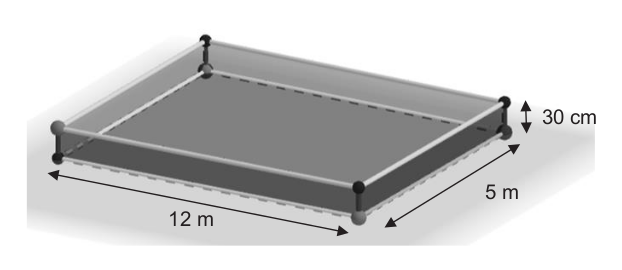
\includegraphics[width=0.8\textwidth]{./images/2022-g3-ex3-img2.png}
\end{center}

\begin{enumerate}
    \item Montrer que le volume de terreau nécessaire pour le potager est de $6$ $m^3$.
    \item Trois magasins proposent les offres suivantes :
    
    \noindent\begin{tabularx}{0.55\linewidth}{|X|}
        \hline
        \\
        {\centering \textbf{Magasin 1}\\}\\
        Livraison : $20$ \euro.\\
        \\
        $0,10$ \euro le litre de terreau.\\
        \\
        \hline         
        \hline
        \\
        {\centering \textbf{Magasin 3}\\}\\
        Livraison offerte pour tout achat supérieur à $50$ \euro.\\
        \\
        $5,37$ \euro le sac de $50$ litres de terreau.\\
        \\
        \hline 
    \end{tabularx}
    \noindent\begin{tabularx}{0.4\linewidth}{|X|}
        \hline
        \\
        {\centering \textbf{Magasin 2}\\}\\
        Livraison offerte.\\
        \\
        $2,35$ \euro le sac de 20 litres de terreau.\\
        \\
        20 \% de remise immédiate après l'achat d’une carte de fidélité au prix de 10 \euro.\\
        \\
        \hline         
    \end{tabularx}
\end{enumerate}

\subsection*{Partie C : Plantation des fleurs}
Dans la perspective d'offrir des bouquets de fleurs pour la fête de l'école, l'enseignante
souhaite planter des graines dans le potager. Dans la classe il y a $26$ élèves et chaque élève
re\c coit $20$ graines à semer.

\medskip
\begin{minipage}{7cm}
    On a reporté ci-contre ce que l’on peut lire sur le paquet de graines choisi.

    \medskip
    On rappelle que le taux de germination d'un paquet de graines indique le pourcentage de graines qui devraient
    germer et donc produire une fleur.
\end{minipage}
\hspace{1cm}
\begin{minipage}{9cm}
    \noindent\begin{tabularx}{0.9\linewidth}{|X|}
        \hline
        \\        
        Taux de germination des graines : $90$ \%\\ 
        \\       
        Prix du paquet de graines : $4,53$ \euro \\
        \\
        Ce paquet contient $50$ graines.\\
        \\
        Période de semis : d'avril à juin\\
        \\
        Hauteur adulte : $50$ cm\\
        \\
        \hline         
    \end{tabularx}
\end{minipage}

\begin{enumerate}
    \item Combien de fleurs un élève peut-il espérer voir pousser ?
    \item Quel sera le budget à prévoir pour l'achat des graines ?
    \item En plus des graines, des bulbes de tulipes et de jonquilles sont plantés.
    \begin{enumerate}
        \item L'enseignante en plante sur un sixième du potager puis un peu plus loin sur un huitième de ce même potager.
        
        Un élève affirme que les bulbes représentent plus de 25 \% du potager. A-t-il raison ?
        
        Justifier votre réponse.
        \item Elle met dans un panier $30$ bulbes de jonquilles et des bulbes de tulipes.
        
        La proportion de bulbes de jonquilles dans le panier est de $\dfrac{5}{6}$.

        Calculer le nombre de bulbes de tulipes dans ce panier.
    \end{enumerate}
\end{enumerate}
